\documentclass[%
	final,
	12pt,
	DIV=11,
	BCOR=4mm,
	twoside=false,
	chapterprefix=true,
	headinclude=true,
	footinclude=true,
	usegeometry=true,
	headings=big,
	headheight=24pt,
	footheight=24pt]{booklet}

\usepackage[top=2.1cm,bottom=2.1cm]{geometry}

\usepackage{commands}
\bibliography{others/booklet.bib}

\hypersetup{
	pdftitle={Booklet},
	pdfauthor={The Author},
	pdfsubject={Booklet, LaTeX, Mathematics},
	pdfkeywords={Booklet, LaTeX, Mathematics}
}

\begin{document}

\begin{titlepage}
	\pagecolor{yellow!70!magenta}\afterpage{\nopagecolor}
	
	{\color{yellow!70!magenta!45!black}
		\parbox[t]{1.1\textwidth}{
			\parbox[t]{1.08\textwidth}{
				\raggedleft
				\fontsize{80pt}{80pt}\selectfont % Fontsize & Line-Spacing
				\textbf{%
					The\\
					Booklet\\
					Template\\
				}
			}
		}
	}
	
	\vfill
	
	\hspace{0.75\textwidth}\colorbox{white}{
		\parbox[t]{0.25\textwidth}{
			\raggedleft\large
			\vspace{2mm} % Top-Padding
			{
				{\Large The Author}\\[4pt]
				1. Auflage\\
			}
			\vspace{2mm} % Bottom-Padding
		}
	}
\end{titlepage}

\frontmatter
\input{others/preface.tex}
\tableofcontents
\mainmatter

\chapter{Übersicht: Beispiel}

\noindent
\begin{center}
	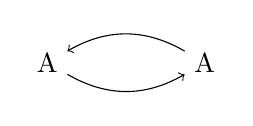
\begin{tikzpicture}
		\node (A) at (-1,0) {A};
		\node (B) at (+1,0) {A};
		\draw [->] (A) to [bend right] (B);
		\draw [->] (B) to [bend right] (A);
	\end{tikzpicture}
	\captionof*{figure}{Diagram}
\end{center}

\appendix

\chapter{Übersicht: Beispiel}

\noindent
\begin{center}
	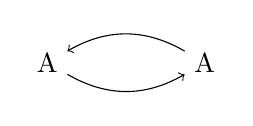
\begin{tikzpicture}
		\node (A) at (-1,0) {A};
		\node (B) at (+1,0) {A};
		\draw [->] (A) to [bend right] (B);
		\draw [->] (B) to [bend right] (A);
	\end{tikzpicture}
	\captionof*{figure}{Diagram}
\end{center}

\backmatter

\chapter{Übersicht: Beispiel}

\noindent
\begin{center}
	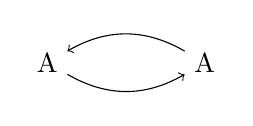
\begin{tikzpicture}
		\node (A) at (-1,0) {A};
		\node (B) at (+1,0) {A};
		\draw [->] (A) to [bend right] (B);
		\draw [->] (B) to [bend right] (A);
	\end{tikzpicture}
	\captionof*{figure}{Diagram}
\end{center}

\printglossaries
\nocite{*}
\addcontentsline{toc}{chapter}{Literaturverzeichnis}
\doublespacing
\printbibliography
\singlespacing
\end{document}
